\section{Endpoint geometry versus global ancestry}\label{sec:endpoint}
For an integer $t$ the endpoint geometry is $K(D(t))$ together with everything determined by $D(t)$ (\cref{prop:P2}). The ancestry of $t$ is its set of complete histories, their classes and their complexes. \cref{prop:P5} separates them.
\begin{proposition}[\SIV{5}: limits of endpoint geometry as a history invariant]\label{prop:P5}\status{new, proved by exhaustive recursion; finite-exact witnesses}
\begin{enumerate}[label=(\alph*),itemsep=1pt]
\item \emph{Obstruction.} $D(900)=D(9000)=\{2,3,5,6,10,15,30\}$, hence $K(D(900))=K(D(9000))$ and all of the data of \cref{prop:P2}(b) coincide, but from the source $4$ there are $2$ histories forming $1$ swap class to $900$ and $4$ histories forming $2$ swap classes to $9000$. Likewise $D(288)=D(4320)$ with $(3\text{ histories},1\text{ class})$ and $(3,2)$ from source $4$.
\item \emph{Consequence.} Neither the number of histories, nor the number of swap classes, nor the isomorphism type of the swap graph of $\Hist(4,t)$ factors through $t\mapsto D(t)$ (\cref{lem:factor}); \emph{a fortiori} none of them factors through $K(D(t))$ or its Betti numbers.
\item \emph{Frequency (finite-exact).} Let $E$ range over the integers $16\le E\le120000$ that are not squarefree and are reachable from the source $4$. They realise $238$ distinct occurrence sets $D(E)$; $166$ of these sets are shared by several $E$, and for $106$ of them the number of swap classes is not constant (for $158$ the number of histories is not constant). This is a finite census and is not extrapolated.
\item \emph{What would suffice.} The fibre sequence $F(h)$ determines the history (\cref{thm:faith-cited}); so the occurrence sets \emph{along the path} reconstruct ancestry, but the occurrence set of the endpoint does not (S2, S3).
\end{enumerate}
\end{proposition}
\begin{proof}
(a) By \cref{prop:P2}(a) the history counts satisfy $H(4,t)=\sum_{d\in D(t)}H(4,t(d-1)/d^2)$; the recursion terminates because predecessors decrease. We evaluated it exactly for $900$ and $9000$ (and for $288,4320$); the $2$ histories to $900$ and the $4$ to $9000$ are listed in Appendix~\ref{app:obstructions}, and the swap classes are computed by union--find over legal adjacent transpositions of those words. $D(900)=D(9000)$ is read off from $900=2^23^25^2$ and $9000=2^33^25^3$: in both, $d^2$ divides the number iff $d\mid30$. (b) is \cref{lem:factor}. (c) is a recorded exhaustive computation (Appendix~\ref{app:finite}). (d) is \cref{thm:faith-cited}.
\end{proof}

\noindent\Cref{fig:endhist} shows endpoint move complex versus history complex.

\begin{figure}[t]\centering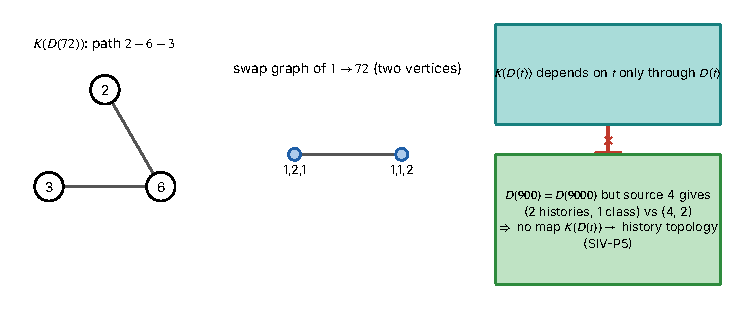
\includegraphics[width=\linewidth]{fig12_endpoint_vs_history.pdf}
\caption{\textbf{Endpoint move complex versus history complex.} Left: $K(D(72))$ is the path $2-6-3$. Middle: the swap graph of the histories $1\to72$ has two vertices. Right: the obstruction \SIV{5}. \emph{Exact; the right panel is schematic.}}\label{fig:endhist}\end{figure}
